\section{Case Study}
\label{section:case_study}

With local schools and libraries closed because of the ongoing global health crisis, we have restricted this preliminary and formative evaluation of Twoville to an individual in our social circles who has served as a beta tester for the Twoville project since November 2020. This individual is a 12-year-old boy who has been paid to proof tutorials, document bugs, design artifacts, and identify missing features. We share a handful of his designs and some of his reflections on his creative process that he shared during interviews.

\subsection{Crabfish}

After the first month, the participant designed an abstract sea creature with pincers and tentacles---naming it {\em crabfish}. After iterating on the design, he arrived upon the shape shown in Figure~\ref{figure:crabfish}, which no longer resembles a fish. To plan out the program, he mentally envisioned a grid and positioned each vertex in relation to its predecessor.

Initially, the participant enumerated every individual vertex position using Cartesian geometry, resulting in a very long program full of hard-coded coordinates. In response to this verbose strategy, we wrote up a tutorial on how to use turtle geometry in Twoville. The participant was already familiar with turtle graphics from other coding platforms. He recast the code as a sequence of moves and turns. Recognizing that the four edges were identical, he wrote code to traverse one edge and wrapped it up in a loop. This version was only a little shorter than the Cartesian approach. We pointed out that there was repetition even within an edge. He then chunked the lines into identical sequences and removed the redundancy using the repeat and repeat-and-a-half loops shown in the figure.

\begin{figure}
\hfill%
\begin{subfigure}{0.45\linewidth}%
\centering
\begin{minipage}{\linewidth}%

\includegraphics[width=\linewidth]{generated/crabfish}
\end{minipage}%
\\
\vspace{0.5em}
\begin{minipage}{0.57\linewidth}%
\small
\begin{Verbatim}
with ungon()
  color = :purple
  formula = :relative
  rounding = 0.05
  with turtle()
    heading = 135
    position = [25, 5]
  repeat 4
    repeat 3
      move().distance = 20
      turn().degrees = 270
    around
      move().distance = 20
      turn().degrees = 90
\end{Verbatim}
\end{minipage}%
\caption{An ungon created using turtle geometry and nested repeat loops.}
\label{figure:crabfish}
\end{subfigure}%
\hfill%
\begin{subfigure}{0.45\linewidth}%
\centering
\begin{minipage}{\linewidth}%

\includegraphics[width=\linewidth]{generated/penrose}
\end{minipage}%
\\
\vspace{0.5em}
\begin{minipage}{0.77\linewidth}%
\small
\begin{Verbatim}
for i to 3
  with polygon()
    color = [0.4 * i, 0.4, 0.9]
    vertex().position = [27, 14]
    vertex().position = [32.5, 30.5]
    vertex().position = [68.8, 37.9]
    vertex().position = [22.2, 87]
    vertex().position = [36.1, 92]
    vertex().position = [92.9, 29.8]
    with rotate()
      pivot = [41, 38]
      degrees = i * 120
    with translate()
      offset = [7, 5]
\end{Verbatim}
\end{minipage}%
\caption{A Penrose triangle created out of three rotations of a template polygon.}
\label{figure:crabfish}
\end{subfigure}%
\hfill%
\caption{Two designs created by the participant.}
\label{figure:penrose}
\end{figure}

\subsection{Penrose}

The participant wished to explore projections of 3D objects into 2D. Initially he intended to make a projection of a rectangular prism, but then he remembered the Penrose triangle illusion. He found an image of it online and observed that it was composed of three interlocking L-shapes. He traced out one of the L-shapes with Twoville's polygon command. To create the other two instances, he embedded the first shape in a loop and applied a rotation transformation. The shapes did not lock together cleanly, so the participant used the direct manipulation handles until he was satisfied with the fit.

\begin{figure}
\begin{minipage}{0.68\linewidth}
\begin{subfigure}{\linewidth}
\begin{minipage}{\linewidth}

\includegraphics[width=\linewidth]{generated/d6}
\end{minipage}%
\caption{The SVG representation exported from Twoville.}
\label{figure:crabfish}
\end{subfigure}%
\vspace{0.5em}
% \vfill
\begin{subfigure}{\linewidth}
\center
\includegraphics[width=\linewidth]{pixels/d6-acrylic}
\caption{The die assembled out of laser-cut acrylic.}
\label{figure:d6_acrylic}
\end{subfigure}
\end{minipage}
\hfill
\begin{subfigure}{0.3\linewidth}
\centering
\begin{minipage}{\linewidth}
\small
\begin{Verbatim}
to tooth()
  move().distance = 2
  turn().degrees = 270
  move().distance = 1
  turn().degrees = 90
  move().distance = 2
  turn().degrees = 90
  move().distance = 1
  turn().degrees = 270
for i to 6
  with polygon()
    opacity = 0
    stroke.color = [1, 0, 0]
    stroke.size = 0.2
    with turtle()
      position = [i * 13 + 12, 2]
      heading = 90
    tooth()
    tooth()
    move().distance = 2
    repeat 2
      move().distance = 1
      turn().degrees = 90
      move().distance = 2
      turn().degrees = 90
      move().distance = 1
      turn().degrees = 270
      tooth()
      tooth()
    turn().degrees = 90
    tooth()
    tooth()
\end{Verbatim}
\end{minipage}
\caption{Twoville source.}
\label{figure:d6_program}
\end{subfigure}%
\caption{A six-sided die designed using turtle geometry and repetition and fabricated by the participant out of a laser-cut acrylic.}
\label{figure:d6}
\end{figure}

\subsection{D6}

The participant occasionally turned to other making activities for design ideas. One of these activities was Perler beads, which are plastic cylinders that are arranged into designs on grids of pegs and melted together using a hot iron. Perler bead creations are usually flat, but the participant had made a series of three-dimensional dice out of them by forming the six faces individually with intermittent beads on their edges to act as joinery. He then snapped the faces together on these interlocking edges. The participant envisioned that the same technique could be used to make a die using a laser cutter and sheets of acrylic. He wrote a Twoville program that mimicked the Perler bead designs he had made earlier. The result is shown in Figure~\ref{figure:d6}.

After writing the first draft of the program, the participant felt that the code was too hard to modify and identified a repeated pattern of moving forward and turning to form a tab. He factored this code out into a function.

Initially the tabs used for the joinery were deeper, exactly mimicking the square grid of Perler beads. We informed the participant that such deep tabs would not be flush with the adjoining faces, and the participant adjusted their depth.

\subsection{Ice Rink}

A logic puzzle in an online math course prompted the participant to create a physical incarnation of the game, as shown in Figure~\ref{figure:icerink}. The board is an ice rink made of discrete cells. The player tries to move the puck into the goal, but inertia carries the puck forward on any movement until it hits an ice block or the wall. The player solves the puzzle by moving the blocks and puck in such a way that the puck stops right on the goal.

The participant started the program by drawing the rink's outer red square with a size of 80. He knew he wanted to place a 5-by-5 grid within this square, along with some padding, so he searched for a cell size that would would get close to 80. He settled on 14 units because the math worked out cleanly. The five cells themselves consumed 70 units, and internal padding between the cells consumed 4 additional units. This left 3 units of padding on each side.

In the online version of the game, the goal is depicted as a star. To make better use of the acrylic material and to make the objective of the game physically clear, the participant formed the puck and goal as concentric circles. Upon cutting, the goal became an annulus, within which the puck comfortably rests.

During the raster-engraving of the cells, which took around ten minutes, the acrylic sheet started to curl upward. The board cooled in this curled state and does not rest flat. The participant is considering ways to prevent this curling, perhaps by making the board smaller, increasing the speed of the laser, or just cutting the cells out completely.

\begin{figure}
\hfill
\begin{minipage}{0.58\linewidth}%
\begin{subfigure}{\linewidth}%
\begin{minipage}{\linewidth}%
\centering
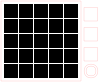
\includegraphics[width=0.7\linewidth]{generated/icerink}%
\end{minipage}
\label{figure:icerink_svg}
\caption{The SVG file exported from Twoville.}
\end{subfigure}%
\vspace{1em}
\\
\begin{subfigure}{\linewidth}
\includegraphics[width=\linewidth]{pixels/icerink-acrylic}%
\label{figure:icerink_photo}
\caption{The game board and pieces fabricated out of acrylic.}
\end{subfigure}%
\end{minipage}%
\hfill
\begin{subfigure}{0.35\linewidth}%
\begin{minipage}{\linewidth}%
\begin{Verbatim}
with rectangle()
  opacity = 0
  stroke.color = [1, 0, 0]
  stroke.size = 0.1
  size = [80, 80]
  corner = [0, 0]
for o to 5
  for i to 5
    with rectangle()
      corner = [3, 3 + i * 15]
      color = [0, 0, 0]
      size = [14, 14]
      with translate()
        offset = [o * 15, 0]
for i to 2  
  with circle()
    stroke.color = [1, 0, 0]
    stroke.size = 0.1
    opacity = 0
    radius = 5 + i * 2
    center = [90, 10]
for i to 3
  with rectangle()
    corner = [83, 20 + i * 20]
    opacity = 0
    stroke.color = [1, 0, 0]
    stroke.size = 0.1
    size = [13.5, 13.5]
\end{Verbatim}
\end{minipage}%
\label{figure:icerink_code}
\caption{Twoville program.}
\end{subfigure}%
\hfill
\caption{An ice rink puzzle game designed by the participant and fabricated out of acrylic.}
\label{figure:icerink}
\end{figure}

\subsection{Interview}
